\documentclass[preview]{standalone}

\usepackage{amsmath}
\usepackage{amssymb}
\usepackage{stellar}
\usepackage{wrapfig}
\usepackage{bettelini}

\hypersetup{
    colorlinks=true,
    linkcolor=black,
    urlcolor=blue,
    pdftitle={Stellar},
    pdfpagemode=FullScreen,
}

\begin{document}

\id{geoeconomica-organizzazioni-internazionali}
\genpage

\section{Forum esclusivi e organizzazioni internazionali}

\begin{snippet}{classificazion-forum-orgainzzazioni-internazionali}
    Un'organizzazione viene detta un forum informale se non è uno statuto giuridico.
    In caso affermativo, se l'organizzazione è statale viene detta
    organizzazione internazionale intergovernative (OIG), altrimenti viene detta
    organizzazione non governative (ONG).
\end{snippet}

\begin{snippetdefinition}{organizzazione-internazionale-intergovernativa-definition}{Organizzazione internazionale intergovernativa}
    Un'\textit{organizzazione internazionale intergovernativa} (OIG) è un'associazione di Stati costituita da un
    trattato (contrariamente alle organizzazioni non governative create da persone private).
    Essa consiste in una persona giuridica distinta da quella degli Stati e funziona grazie a degli organi comuni
    previsti dai suoi statuti.
\end{snippetdefinition}

\begin{snippet}{2627a7a1-bd3c-4131-beb1-201e8624724c}
    È dunque una struttura di cooperazione tra Stati che persegue degli scopi di
    interesse comune definiti nel suo atto costitutivo.
    L'organizzazione internazionale è il simbolo dell'evoluzione delle relazioni internazionali. Gli Stati
    sono maestri del gioco poiché essi hanno il potere di creare delle organizzazioni internazionali, ma
    le loro creature rischiano di sfuggire al loro controllo. Se gli Stati, specialmente quelli più potenti,
    controllano le organizzazioni con l'arma efficace del contributo finanziario, essi non hanno più il monopolio delle relazioni internazionali.
    Si distinguono due forme di organizzazioni governative: quelle \quotes{universali} e quelle \quotes{regionali}.
\end{snippet}

% https://moodle.edu.ti.ch/libe/pluginfile.php/122248/mod_resource/content/0/Pass_06f_OrganizzazioniEForum_23-24_schede.pdf

\section{ONU}

\begin{snippetdefinition}{onu-definition}{Organizzazione delle Nazioni Unite}
    L'\textit{Organizzazione delle Nazioni Unite}
    è un'organizzazione intergovernativa a carattere mondiale.
    Tra i suoi obiettivi principali vi sono il mantenimento della pace e
    della sicurezza mondiale, lo sviluppo di relazioni amichevoli tra le nazioni,
    il perseguimento di una cooperazione internazionale e il favorire
    l'armonizzazione delle varie azioni compiute a questi scopi dai suoi membri.
\end{snippetdefinition}

% multilateralismo

\begin{snippet}{onu-componenti}
    L'ONU è composto da diversi componenti:
    \begin{itemize}
        \item \textbf{Assemblea generale:}
            È il principale organo deliberativo dell'ONU, dove sono rappresentati
            tutti gli Stati membri. Ogni Stato ha un voto.
            L'Assemblea Generale discute e adotta risoluzioni su questioni rilevanti per
            la pace e la sicurezza, lo sviluppo internazionale, i diritti umani e
            altri temi globali.
        \item \textbf{Consiglio di Sicurezza:}
            è responsabile del mantenimento della pace e della
            sicurezza internazionali.
            È composto da 15 membri, di cui 5 permanenti con diritto di veto
            (Stati Uniti, Regno Unito, Francia, Russia, Cina) e 10 non permanenti eletti
            per periodi di due anni. Il Consiglio di Sicurezza può autorizzare
            operazioni di pace, sanzioni e azioni militari.
        \item \textbf{Segretariato:}
            è l'organo amministrativo dell'ONU. Il Segretario Generale
            è il capo del Segretariato. Questo organo esegue il lavoro quotidiano dell'ONU e implementa le decisioni degli altri organi.
    \end{itemize}
    e altri ancora.
\end{snippet}

\plain{La Svizzera è entrata nell'ONU nel 2002.}

\begin{snippetdefinition}{diritto-di-veto-definition}{Diritto di veto}
    Con \textit{diritto di veto} si intende
    potere riconosciuto al membro di \underline{un} organo deliberante di bloccarne una decisione. 
\end{snippetdefinition}

\begin{snippet}{problema-onu-veto}
    L'ONU si ritrova spesso con la mani legate in quanto
    molte decisioni vengono bloccate dai diritti di veto, che incrociandosi
    bloccano molte iniziative.
    Il diritto di veto è esso stesso soggetto al diritto di veto, in quanto
    la sua rimozione dovrebbe essere presa dal consiglio di sicurezza.
\end{snippet}

\begin{snippet}{onu-riassunto}
    \vspace{-0.5cm}
    \setlength{\intextsep}{0pt}%
    \begin{wrapfigure}{l}{.25\textwidth}
        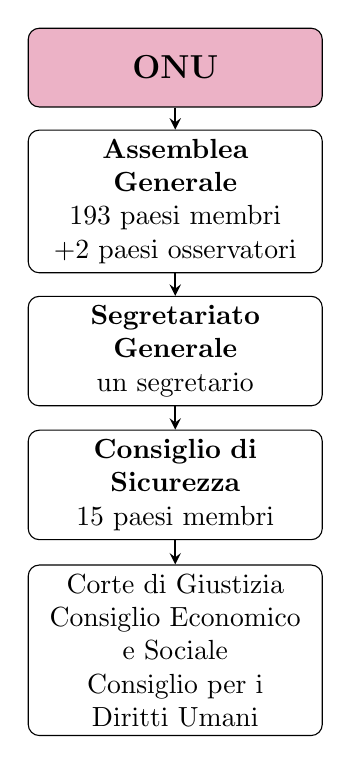
\begin{tikzpicture}
            \tikzstyle{box} = [rectangle, rounded corners, minimum width=3cm, minimum height=1cm, text centered, draw=black, fill=white, text width=3.5cm, align=center]
            \tikzstyle{arrow} = [thick,->,>=stealth]
        
            % Nodes
            \node (onu) [box, fill=purple!30] {\large \textbf{ONU}};
            \node (assemblea) [box, below of=onu, node distance=1.7cm] {\textbf{Assemblea Generale}\\193 paesi membri\\+2 paesi osservatori};
            \node (segreteria) [box, below of=assemblea, node distance=1.9cm] {\textbf{Segretariato Generale}\\un segretario};
            \node (sicurezza) [box, below of=segreteria, node distance=1.7cm] {\textbf{Consiglio di Sicurezza}\\15 paesi membri};
            \node (giustizia) [box, below of=sicurezza, node distance=2.1cm] {Corte di Giustizia\\Consiglio Economico\\e Sociale\\Consiglio per i Diritti Umani};
        
            % Arrows
            \draw [arrow] (onu) -- (assemblea);
            \draw [arrow] (assemblea) -- (segreteria);
            \draw [arrow] (segreteria) -- (sicurezza);
            \draw [arrow] (sicurezza) -- (giustizia);
        \end{tikzpicture}
        \vspace{-2.4cm}
    \end{wrapfigure}
    
    L'ONU nasce nel 1920 come ``Società delle Nazioni'', con lo scopo quello di accrescere il
    benessere e la qualità della vita degli esseri umani.
    La Società delle Nazioni cesserà la sua attività nel 1946, a seguito della Seconda guerra
    mondiale, e verrà sostituita dall'ONU, attiva tutt'oggi, aggiungendo però ai suoi scopi anche
    il garantire la pace e la sicurezza nel mondo, oltre a promuovere lo sviluppo sostenibile.
    
    \textbf{Obiettivi:} Garantire pace e sicurezza nel mondo e promuovere lo sviluppo
        sostenibile.
    
    \textbf{Membri:} 193 paesi + 2 osservatori (Vaticano e Palestina).
    
    \textbf{Consiglio di sicurezza:} 15 paesi membri, dei quali 5 permanenti e 10 in rotazione.
    
    \textbf{Ruolo della Svizzera:} CH è un membro dell'ONU dal 2002.\\
        Dal 2023 al 2024 occupa un seggio non permanente nel Consiglio di sicurezza.
    
    \textbf{Diritto di veto:} Diritto di opposizione a una legge alla decisione finale.
    \wrapfill
    \vspace{1.5cm}
\end{snippet}

\section{L'Unione Europea}

\begin{snippetdefinition}{comunita-europeacarbone-acciaio-definition}{Comunità europea del carbone e dell'acciaio}
    La \textit{Comunità europea del carbone e dell'acciaio} (CECA)
    fu creata col Trattato di Parigi del 18 aprile 1951
    con lo scopo di mettere in comune le produzioni di queste due materie prime in un'Europa
    di sei paesi: Belgio, Francia, Germania Occidentale, Italia, Lussemburgo e Paesi Bassi.
    Era concepita come passo iniziale di un processo federale europeo.
\end{snippetdefinition}

\begin{snippet}{ceca-expl1}
    La CECA fu l'istituzione che precorse
    la strada del Trattato di Roma, con il quale venne
    costituita la Comunità economica europea, divenuta Unione europea nel 1992.
    L'Unione Europea, nonostante ricopra solo parte dell'Europa, ha comunque una grande influenza globale.
\end{snippet}

% 2 esempi
% Politica agricola europea
% Fondo europea di sviluppo regionale

\subsection{Relazione fra Svizzera e Unione Europea}

\begin{snippetdefinition}{accordi-bilanterali-definition}{Accordi bilaterali}
    Nel 1999 la Svizzera e l'Unione Europea (UE) hanno concluso sette accordi
    bilaterali (conosciuti come \textit{Bilaterali I}),
    che sono stati approvati dal popolo svizzero nel 2000.
    Gli accordi disciplinano le relazioni tra la Svizzera e l'UE nei settori
    della libera circolazione delle persone,
    dei trasporti terrestri, dei trasporti aerei, degli
    ostacoli tecnici al commercio, degli acquisti pubblici,
    della ricerca e dell'agricoltura.
\end{snippetdefinition}

\begin{snippet}{relazione-svizzera-ue}
    Gli accordi sono connessi giuridicamente tra di loro per mezzo della cosiddetta
    «clausola ghigliottina»:
    se una delle parti contraenti dovesse denunciare uno degli accordi settoriali,
    decadono automaticamente anche i restanti accordi.
    \\\\
    I Bilaterali I rappresentano una base importante per le relazioni
    tra la Svizzera e l'UE: contribuiscono ad assicurare
    la crescita economica a medio-lungo termine e a
    creare posti di lavoro, garantendo alle persone e alle
    imprese svizzere le stesse condizioni di accesso al mercato
    interno europeo di cui godono gli altri Stati membri dell'UE.
    Inoltre, gli accordi promuovono il costante rafforzamento dei
    rapporti tra la Svizzera e l'UE a tutti i livelli.
\end{snippet}

\begin{snippetdefinition}{accordo-schengen-definition}{Accordo di Schengen}
    L'\textit{accordo di Schengen} è un trattato internazionale firmato a
    Schengen il 14 giugno 1985 tra Benelux, Germania Ovest e Francia,
    che prevedeva la creazione di uno spazio comune, tramite una progressiva eliminazione
    dei controlli alle frontiere comuni tra i cinque Stati interessati,
    sia delle merci sia delle persone.
    \\
    L'accordo è stato il primo passo del cosiddetto acquis di Schengen,
    che dal 1999 è stato integrato nel quadro istituzionale e
    giuridico dell'Unione europea.
\end{snippetdefinition}

\begin{snippetdefinition}{convenzione-dublino-definition}{Convenzione di Dublino}
    La Convenzione sulla determinazione dello stato competente per l'esame di una domanda di asilo presentata
    in uno degli stati membri della Comunità Europea,
    comunemente conosciuta come Convenzione di Dublino, è un trattato
    internazionale multilaterale in tema di diritto di asilo. 
\end{snippetdefinition}

\begin{snippet}{svizzera-accordo-dublino-schengen}
    La Svizzera, pur non facendo parte dell'Unione Europa, possiede dei contratti di
    cooperazione con l'accordo di Dublino e di Schengen.
\end{snippet}

\begin{snippet}{7b07b404-d98d-4af3-aa3a-93a9e4969ccb}
    L'accordo di Dublino viene indotto dall'accordo di Schengen, in quanto
    i richiedenti di asilo potrebbero spostarsi da nazione a nazione senza
    essere controllato alla dogana. I sistemi informatici per le richieste d'asilo sono
    condivisi.
\end{snippet}

\section{Altre organizzazioni}

\begin{snippetdefinition}{unesco-definition}{UNESCO}
    L'\textit{UNESCO} (Organizzazione delle Nazioni Unite per l'Educazione, la Scienza e la Cultura) si occupa di
    promuovere l'educazione, il patrimonio culturale e la collaborazione scientifica a livello internazionale.
\end{snippetdefinition}

\begin{snippetdefinition}{g7-definition}{G7}
    \textit{G7} (Gruppo dei Sette) è un forum informale di sette grandi economie avanzate del mondo, che discutono
    e cooperano su questioni economiche globali.
\end{snippetdefinition}

\begin{snippetdefinition}{wef-definition}{WEF}
    Il \textit{WEF} (World Economic Forum) è una organizzazione internazionale per la cooperazione pubblico-privato che
    si incontra annualmente a Davos, in Svizzera, per discutere le principali questioni economiche globali.
\end{snippetdefinition}

\begin{snippetdefinition}{wto-definition}{WTO}
    Il \textit{WTO} (World Trade Organization) è una organizzazione internazionale che si occupa delle regole del commercio
    tra le nazioni con l'obiettivo di assicurare che i flussi commerciali procedano il più possibile agevolmente,
    prevedibilmente e liberamente possibile.
\end{snippetdefinition}

\begin{snippetdefinition}{g20-definition}{G20}
    Il \textit{G20} (Gruppo dei Venti) è un forum internazionale che riunisce le 19 economie più grandi del mondo più
    l'Unione Europea. Si occupa di politica economica e finanziaria.
\end{snippetdefinition}

\begin{snippetdefinition}{amnesty-international-definition}{Amnesty International}
    \textit{Amnesty International} è una organizzazione non governativa che si occupa di diritti umani con l'obiettivo di
    fare ricerca e azione per prevenire e porre fine a gravi abusi dei diritti civili.
\end{snippetdefinition}

\begin{snippetdefinition}{wwf-definition}{WWF}
    Il \textit{WWF} (World Wide Fund for Nature) organizzazione non governativa internazionale che si occupa della
    conservazione, ricerca e ripristino dell'ambiente naturale.
\end{snippetdefinition}

\end{document}